\begin{titlepage}
\newgeometry{margin=0pt}
\thispagestyle{empty}
\begin{tikzpicture}[remember picture,overlay]
  \node[anchor=south west,inner sep=0pt] at (current page.south west) {%
    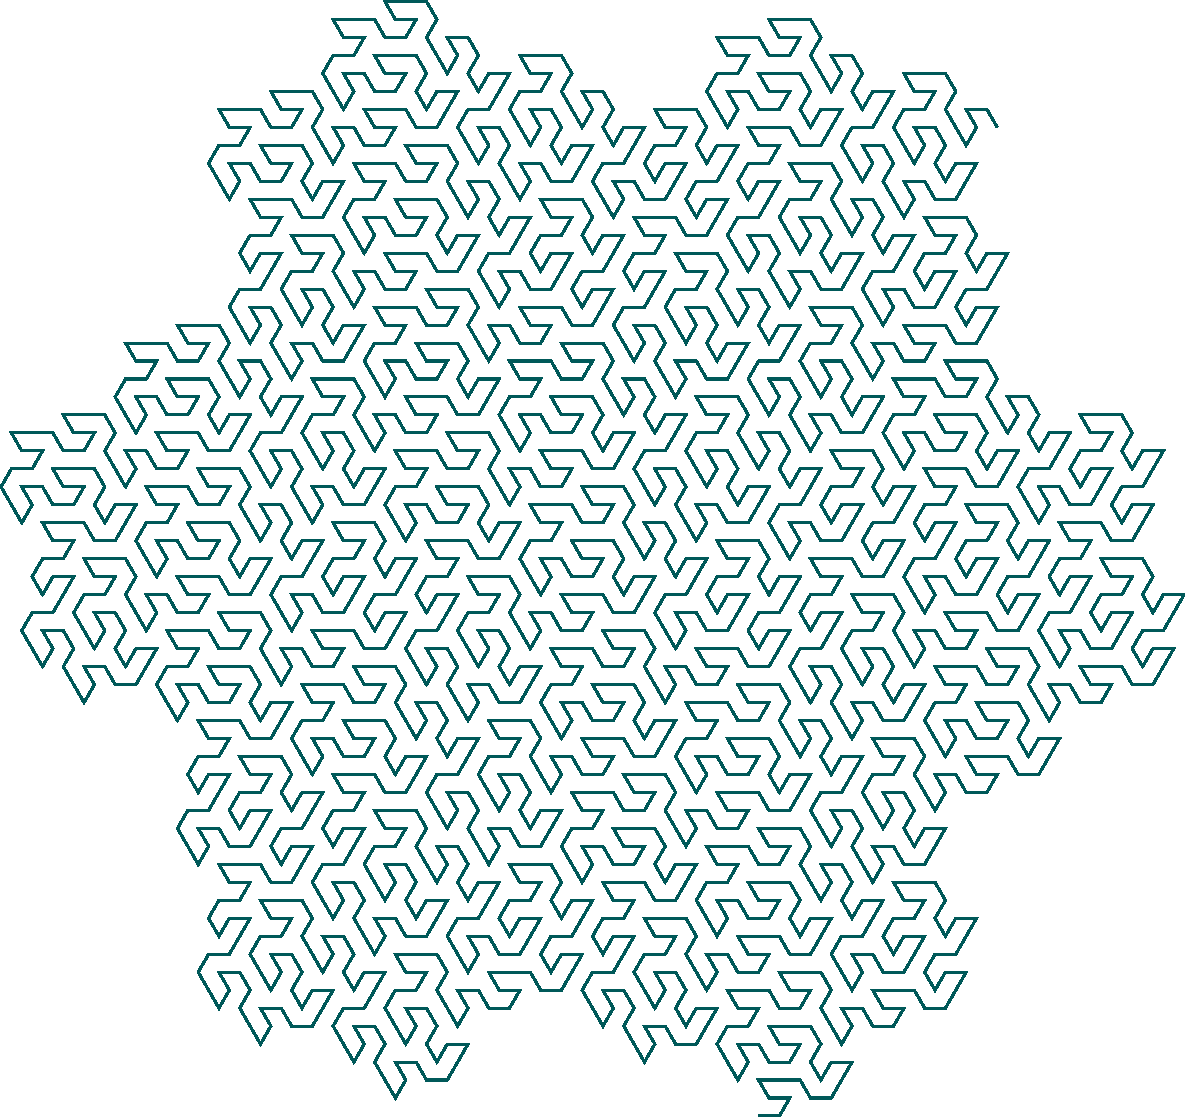
\includegraphics[width=\paperwidth,height=\paperheight]{assets/matte-generator.pdf}%
  };
  \fill[black,opacity=0.3]
    (current page.south west) rectangle (current page.north east);
  \node[
    align=center,
    text=white,
    fill=black,
    fill opacity=0.45,
    text opacity=1,
    rounded corners=2pt,
    inner xsep=10pt,
    inner ysep=8pt
  ] at (current page.center) {%
    \begin{minipage}{0.86\paperwidth}
      \centering
      \HSCMatteTitleText
        {Extension and Specialist Mathematics}
        {AUS-Networks\\[0.2cm]\Large An Introduction to Graph Theory}
        {Vu Hung Nguyen}
    \end{minipage}%
  };
\end{tikzpicture}
\null
\restoregeometry
\end{titlepage}